\documentclass[12pt,a4paper]{article}
\usepackage{graphicx}
\usepackage{amsmath}
\usepackage{amssymb}
\usepackage{listings}
\usepackage{geometry}
\usepackage{multicol}
\geometry{margin=1in}
\begin{document}
\noindent

\begin{minipage}{0.6\textwidth}

\includegraphics[width=0.75\textwidth]{IIITB-COMET-Logo.png}
\end{minipage}
\begin{minipage}{0.38\textwidth}
\begin{center}
\textbf{DARSI VAMSI}
\newline
\textbf{COMET FWC 071}
\end{center}
\end{minipage}
\newline
\newline
\begin{center}
    {\LARGE\textbf{Implementation of the Boolean Function}}\\[0.3cm]
    {\LARGE\textbf{$Y=AB+CD$ Using Raspberry Pi Pico 2 W with 7Segment Dsiplay }}
    \\
    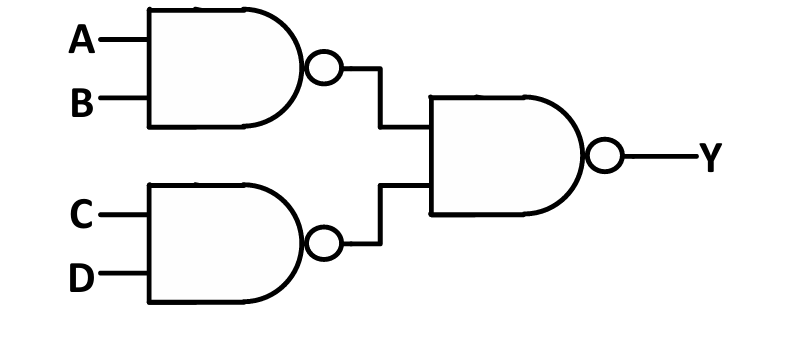
\includegraphics[width=0.75\textwidth]{figure.png}
\end{center}

\section{Problem Analysis}

The given logic circuit consists of three NAND gates.

The output of the first NAND gate is

$$
X_1=(AB)'
$$

The output of the second NAND gate is

$$
X_2=(CD)'
$$

The final output is

$$
Y=(X_1X_2)'
$$

Substituting the values of $X_1$ and $X_2$,

$$
Y=((AB)'(CD)')'
$$

Applying De Morgan's theorem,

$$
Y=((AB)')'+((CD)')'
$$

Therefore,

$$
\boxed{Y=AB+CD}
$$

The output becomes logic '1' whenever:

\begin{itemize}
    \item $A=1$ and $B=1$, or
    \item $C=1$ and $D=1$.
\end{itemize}
\section{Hardware Requirements}

\begin{tabular}{|c|l|}
\hline
\textbf{S.No} & \textbf{Component Name} \\
\hline
1 & Raspberry Pi Pico 2W \\
2 & 7-Segment Display (Common Cathode/Anode) \\
3 & Breadboard \\
4 & Jumper Wires \\
5 & Resistors (220$\Omega$ – 330$\Omega$) \\
6 & USB Cable / 5V Power Supply \\
7 & Logic Level Shifter (Optional) \\
\hline
\end{tabular}

\section{Pin Connections}

\subsection*{7-Segment Display Connections}

\begin{tabular}{|c|c|c|}
\hline
\textbf{7-Segment Pin} & \textbf{Segment} & \textbf{Pico GPIO Pin} \\
\hline
a & Segment A & GP0 \\
b & Segment B & GP1 \\
c & Segment C & GP2 \\
d & Segment D & GP3 \\
e & Segment E & GP4 \\
f & Segment F & GP5 \\
g & Segment G & GP6 \\
\hline
\end{tabular}

\subsection*{Internal Inputs}

The inputs $A, B, C, D$ are generated internally in the program to evaluate the Boolean expression:
\[
Y = (A \cdot B) + (C \cdot D)
\]
Otherwise, the output remains logic '0'.
\section{Hardware Setup and Accessing Raspberry Pi Pico 2 W Using Arduino IDE}

The Raspberry Pi Pico 2 W is programmed using the Arduino IDE by installing the necessary board support packages and configuring the development environment. The detailed procedure is as follows.



\subsection{Installing Arduino IDE}

\begin{enumerate}
    \item Download and install the latest version of Arduino IDE from the official Arduino website.
    \item Open the Arduino IDE after installation.
\end{enumerate}

\subsection{Installing Raspberry Pi Pico 2 W Board Package}

\begin{enumerate}
    \item Open Arduino IDE.
    \item Navigate to
    $$
    \text{File} \rightarrow \text{Preferences}
    $$
    \item In the ``Additional Boards Manager URLs'' field, add the following URL:
    
\begin{verbatim}
https://github.com/earlephilhower/arduino-pico/releases/download/global/package_rp2040_index.json
\end{verbatim}

    \item Click ``OK''.
    
    \item Navigate to
    \[
    \text{Tools} \rightarrow \text{Board} \rightarrow \text{Boards Manager}
    \]

    \item Search for ``Raspberry Pi Pico/RP2040''.

    \item Install the package developed by Earle F. Philhower.
\end{enumerate}

\subsection{Connecting the Raspberry Pi Pico 2 W}

\begin{enumerate}
    \item Connect the Raspberry Pi Pico 2 W to the computer using a USB Type-C cable.
    
    \item If the board is not detected automatically:
    \begin{enumerate}
        \item Press and hold the \textbf{BOOTSEL} button.
        \item Connect the USB cable while holding the button.
        \item Release the button after the board appears as a removable drive.
    \end{enumerate}
\end{enumerate}

\subsection{Selecting the Board and Port}

\begin{enumerate}
    \item Navigate to
    \[
    \text{Tools} \rightarrow \text{Board}
    \]

    \item Select
    \[
    \text{Raspberry Pi Pico 2 W}
    \]

    \item Navigate to
    \[
    \text{Tools} \rightarrow \text{Port}
    \]

    \item Select the corresponding COM port of the Raspberry Pi Pico 2 W.
\end{enumerate}

\subsection{Uploading the Program}

\begin{enumerate}
    \item Write or paste the Arduino program into the Arduino IDE.
    \item Click the \textbf{Verify} button to compile the code.
    \item Click the \textbf{Upload} button.
    \item Wait until the message

Done Uploading\\
appears in the output window.
\end{enumerate}


After successful uploading of the program, the Raspberry Pi Pico 2 W executes the Boolean expression

$$
Y = AB + CD
$$

for all possible input combinations and displays the output through the LED connected to GP1.
\section{Results}

The Raspberry Pi Pico 2W successfully evaluates the Boolean function and displays the output on the 7-segment display.

\subsection*{Observation Table}

\begin{tabular}{|c|c|c|c|c|c|}
\hline
\textbf{A} & \textbf{B} & \textbf{C} & \textbf{D} & \textbf{Y = AB + CD} & \textbf{Display} \\
\hline
0 & 0 & 0 & 0 & 0 & 0 \\
1 & 1 & 0 & 0 & 1 & 1 \\
0 & 0 & 1 & 1 & 1 & 1 \\
1 & 0 & 1 & 0 & 0 & 0 \\
\hline
\end{tabular}
\begin{multicols}{2}
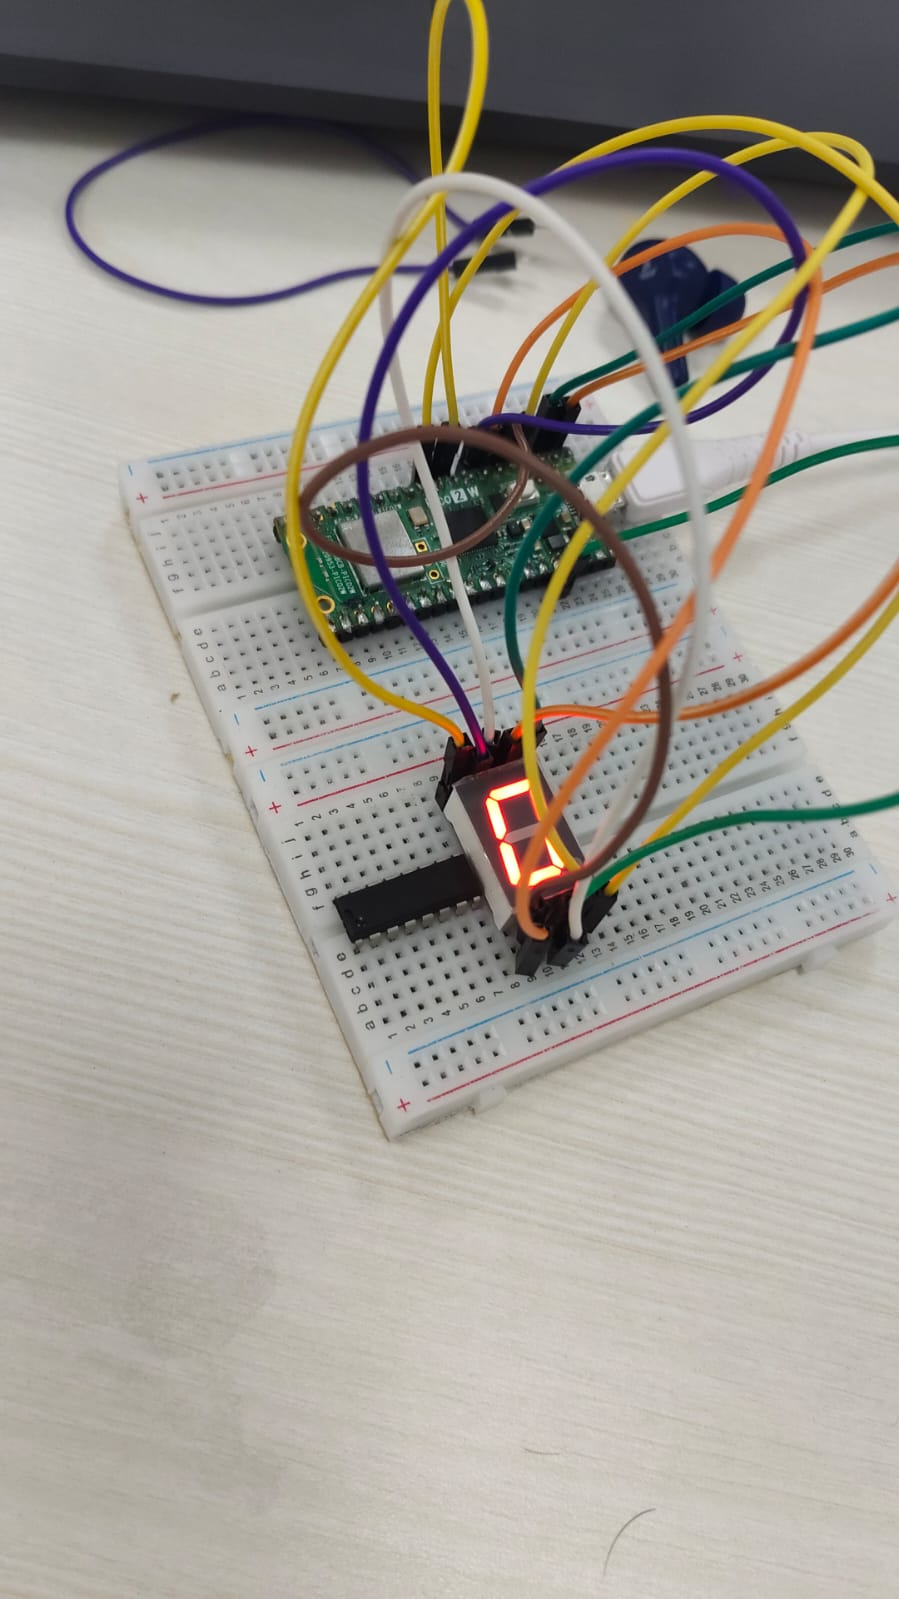
\includegraphics[width=0.2\textwidth]{output as zero.jpeg}
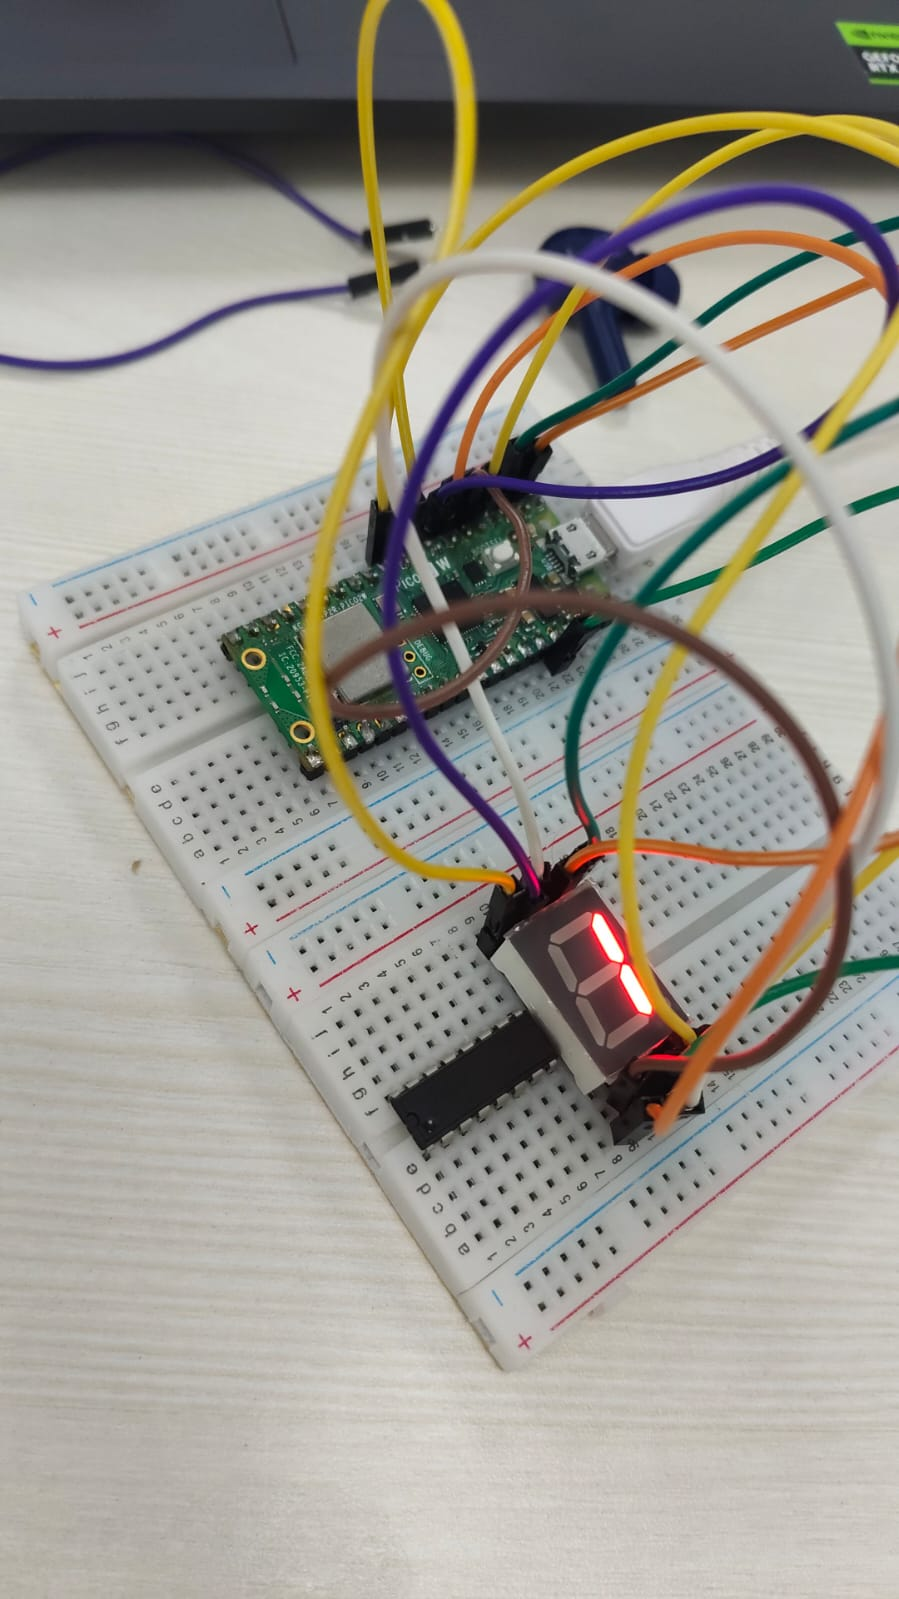
\includegraphics[width=0.2\textwidth]{Output as one (2).jpeg}
\end{multicols}
\end{document}